\documentclass[final,t,overlay]{beamer}
\mode<presentation>
{
  \usetheme{UCL}
}
\usepackage[size=a0,scale=1,debug]{beamerposter}

% additional packages
\usepackage[english]{babel}
\usepackage[utf8]{inputenc}
\usepackage{pstool}
\usepackage{calc}
\usepackage{import}
\usepackage{color}
\usepackage{multicol}
\usepackage{graphicx}
\usepackage{tikz}
\usepackage{amsmath}
\usepackage{amsthm,amsthm}
\usepackage{amssymb}
\usetikzlibrary{arrows,shapes}
\tikzstyle{square}=[draw, minimum size=2.5em]
\tikzstyle{round}=[draw,circle, minimum size=2.5em]

 \def\mm#1{\ensuremath{\boldsymbol{#1}}} % version: amsmath
 
\DeclareMathOperator{\diag}{diag}
\DeclareMathOperator{\var}{var}
\DeclareMathOperator{\med}{Median}
\DeclareMathOperator{\chol}{cholesky}
\DeclareMathOperator{\tr}{tr}
\DeclareMathOperator*{\minimise}{minimise}
\DeclareMathOperator*{\argmax}{arg\,max}
\DeclareMathOperator*{\argmin}{arg\,min}

\global\long\def\Mz{M_{\mathbf{z},y}}
\global\long\def\muz{\mu_{\mathbf{z}}}
\global\long\def\aj{\alpha^{(j)}}
\global\long\def\ajt{\left(\alpha^{(j)}\right)^{\top}}

%empf is red now
%\renewcommand{\emph}[1]{{\color{red}{#1}}}

\title{A Kernel Test of Goodness of Fit}
\author[SHORTAUTHOR]
{Kacper Chwialkowski$^*$ Heiko Strathmann$^*$ Arthur Gretton}
\institute[SHORTINSTITUTE]{Gatsby Unit, University College London.}

\date[SHORTDATE]{DATE}

\global\long\def\ev{\mathbb{E}}

\newtheorem{thm}{Theorem}
\definecolor{mg}{rgb}{0,0.44,0}
\usepackage{graphicx}


\begin{document}
\begin{frame}
\begin{columns}
\begin{column}{.33\linewidth}
\vspace{-0.75cm}
\begin{block}{Motivation: One sample testing for non i.i.d.\ data}
\begin{minipage}{.57\linewidth}
\begin{itemize}
\item TODO Intro
\end{itemize}
\end{minipage}
\begin{minipage}{.37\linewidth}
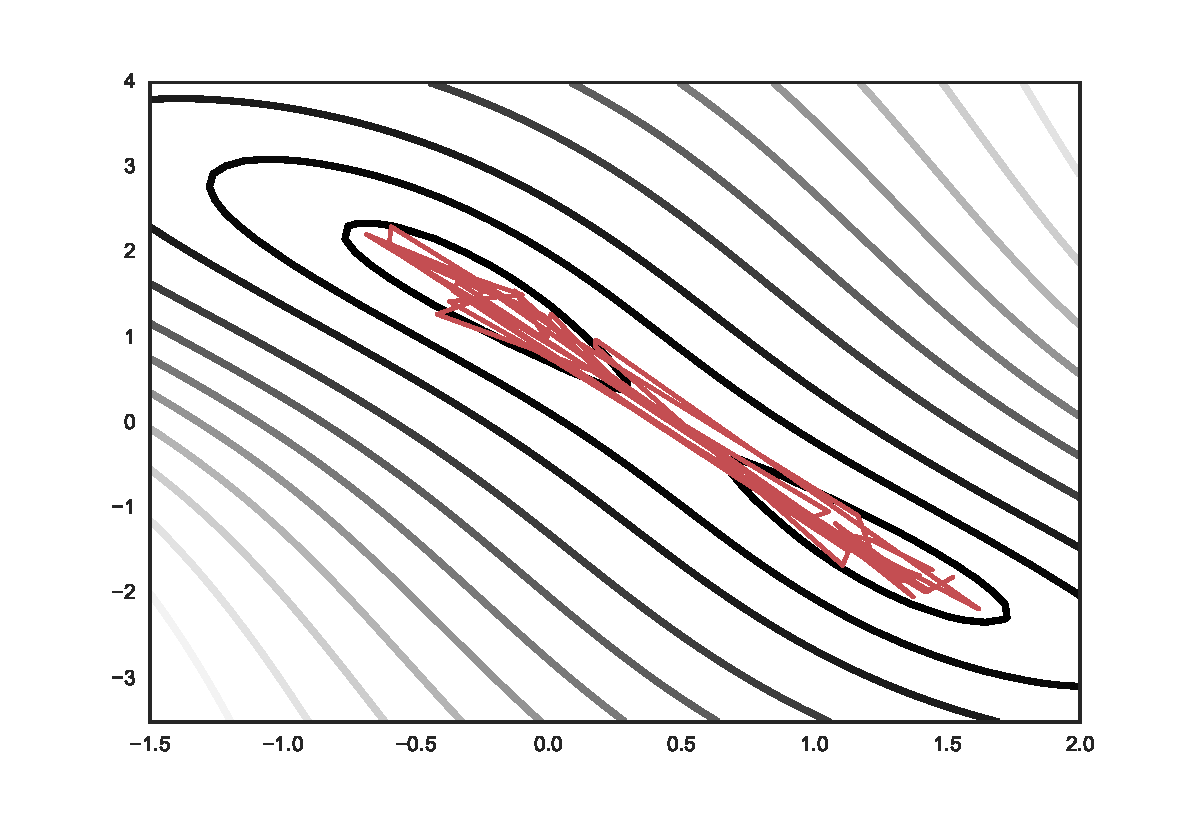
\includegraphics[scale=0.8]{img/sgld_trace_and_density.pdf}
\end{minipage}
\vspace{1cm}
\begin{center}
\emph{Punch line 1}
\end{center}
\end{block}
\vspace{-0.75cm}
\begin{block}{So far: Maximum Mean Discrepancy}
\begin{center}Idea: Function in RKHS to reveal difference in distributions\end{center}
\begin{minipage}{.60\linewidth}
\begin{itemize}
\item Cite paper?
\item Intuition MMD
\end{itemize}
\end{minipage}
\begin{minipage}{.35\linewidth}
\begin{center}
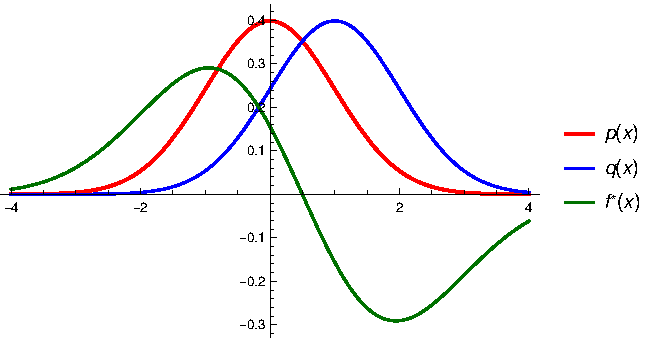
\includegraphics[width=12cm,height=6cm]{./img/mmd.pdf}
\end{center}
\end{minipage}
\vspace{1cm}
\begin{center}
\emph{Can we do this without sampling from $p$?}
\end{center}
\end{block}
\vspace{-0.75cm}
\begin{block}{Stein's trick in RKHS}
\begin{itemize}
\item Get rid of $\ev_{{\color{red} p}}f$  in
\begin{align*}
\sup_{f \in F} [\ev_{{ \color{blue} q}}f - \ev_{{\color{red} p}} f ]
\end{align*}
 \item Consider the  class $G = \{ f  +  \log' { \color{blue} q} \cdot  f | f \in F \}$ justified by 
\begin{align*}
 0= &  f(x) {\color{red} p}(x)  \big|_{x=-\infty}^{x=\infty} \\
   = &  \int_{-\infty}^{\infty} (f(x) {\color{red} p}(x) )'  dx \\
   = &  \int   f(x)' { \color{blue} q}(x)   + f(x){\color{red} p}'(x)  \\
   = &  \ev_{\color{red} p} f(X)  +  \log' {\color{red} p}(X) f(X) \\
   = & \ev_{\color{red} p} g(X), \\
    & \quad \quad \quad  \quad  \text{ where } g \in G
\end{align*}
\end{itemize}
\end{block}
\vspace{-0.75cm}
\begin{block}{Stein discrepancy}
 \begin{align*}
G = \{ f  +  \log' {\color{red} p} f | f \in F \}
\end{align*}
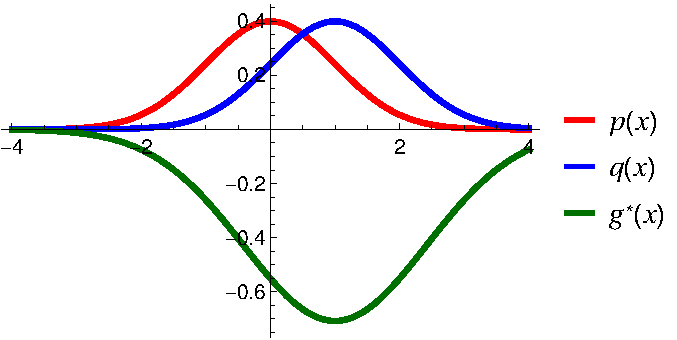
\includegraphics[scale=1]{./img/s1.pdf}
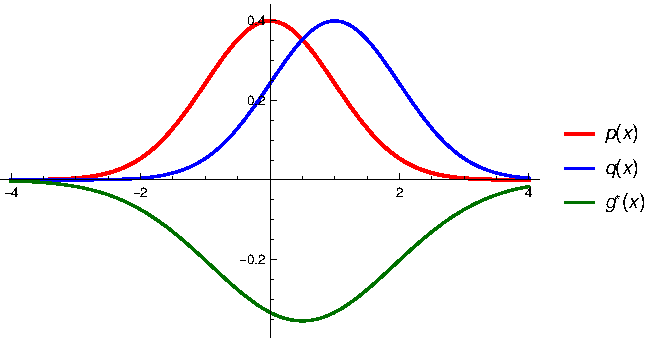
\includegraphics[scale=1]{./img/s05.pdf}
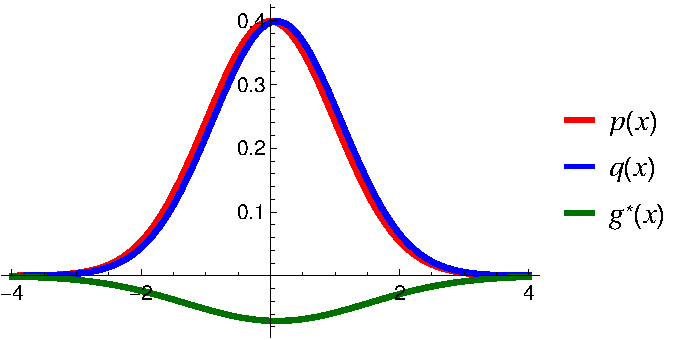
\includegraphics[scale=1]{./img/s01.pdf}

%%\includegraphics[width=10cm, height=7cm]{./img/old/figures/kmc/gaussian_trajectories_momentum_hmc}
%\includegraphics[scale=1.2]{./img/old/figures/kmc/gaussian_trajectories_acceptance_hmc}\\

%\includegraphics[scale=.5]{./img/old/figures/kmc/kmc_banana_bbox}
%%\includegraphics[width=10cm, height=7cm]{./img/old/figures/kmc/gaussian_trajectories_momentum_kmc}
%\includegraphics[scale=1.2]{./img/old/figures/kmc/gaussian_trajectories_acceptance_kmc}
\vspace{1cm}
\begin{center}
\emph{Bam!}
\end{center}
\end{block}
\end{column}

%%%-----------------column 2
\hspace{-1.45cm}
\begin{column}{.33\linewidth}

\vspace{-0.75cm}
\begin{block}{Closed form expression}
 Let $F$ be the RKHS associated with the kernel $k$. Consider a friendly looking function
\begin{align*}
h_{{\color{red} p}}(x,y) & := \partial_{x} \log {\color{red} p}(x) \partial_{x} \log {\color{red} p}(y) k(x,y)\\
 & \quad+\partial_{y} \log {\color{red} p}(y) \partial_{x}  k(x,y)\\
 & \quad+\partial_{x} \log {\color{red} p}(x) \partial_{y}k(x,y)\\
 & \quad+\partial_{x} \partial_{y} k(x,y).
\end{align*}
 \center{\emph{Only depends on kernel and $\partial_{x} \log {\color{red} p}(x)$}}
 
\end{block}

\vspace{-0.75cm}
\begin{block}{Theorem}
Let ${ \color{blue} q},{\color{red} p}$ be probability measures and $Z\sim { \color{blue} q}$. 
If $\ev_{{ \color{blue} q}} h_{{\color{red} p}}(Z,Z)<\infty$, then $MMD({\color{red} p},{ \color{blue} q},G) = \ev_{{ \color{blue} q}} h_{{\color{red} p}}(Z,Z')$.
\end{block}
\vspace{-0.75cm}
\begin{block}{Theorem}
 If the kernel $k$ is cc-universal, $\ev_{{ \color{blue} q}} h_{{ \color{blue} q}}(Z,Z)<\infty$ and $\ev_{{ \color{blue} q}} (\log' \frac{{\color{red} p}(Z)}{{ \color{blue} q}(Z)})^{2}<\infty$
then $MMD({\color{red} p},{ \color{blue} q},G) =0$ if and only if ${\color{red} p}={ \color{blue} q}$.

\end{block}
\vspace{-0.75cm}
\begin{block}{Estimation: V-statistics}
An estimator of $\ev h_{\color{red} p}(X,X')$ is
\begin{align*}
 V_n(h_{\color{red} p}) = \frac {1} {n^2} \sum_{i,j=1}^n h_{\color{red} p}(X_i,X_j).
\end{align*}
Our test statistic is $ n V_n(h_{\color{red} p})$.

If $X_i \sim {\color{red} p}$ then $ n V_n(h_{\color{red} p})$  converges weakly. 

Otherwise it does not,  it explodes, $P(n V_n(h_{\color{red} p}) <C) \to 0$.
\end{block}
\vspace{-0.75cm}
\begin{block}{Non i.i.d.\ extension: the wild bootstrap}
To estimate quantiles of $ V_n(h_{\color{red} p})$  
\[
 V_n(h_{\color{red} p}) = \frac {1} {n^2} \sum_{i,j=1}^n h_{\color{red} p}(X_i,X_j).
\]
under the null, we use wild bootstrap
\[
 B_n(h_{\color{red} p}) = \frac {1} {n^2} \sum_{i,j=1}^n W_i W_j h_{\color{red} p}(X_i,X_j).
\]
  where $W_i$ is a specific series of zero valued random variables.


 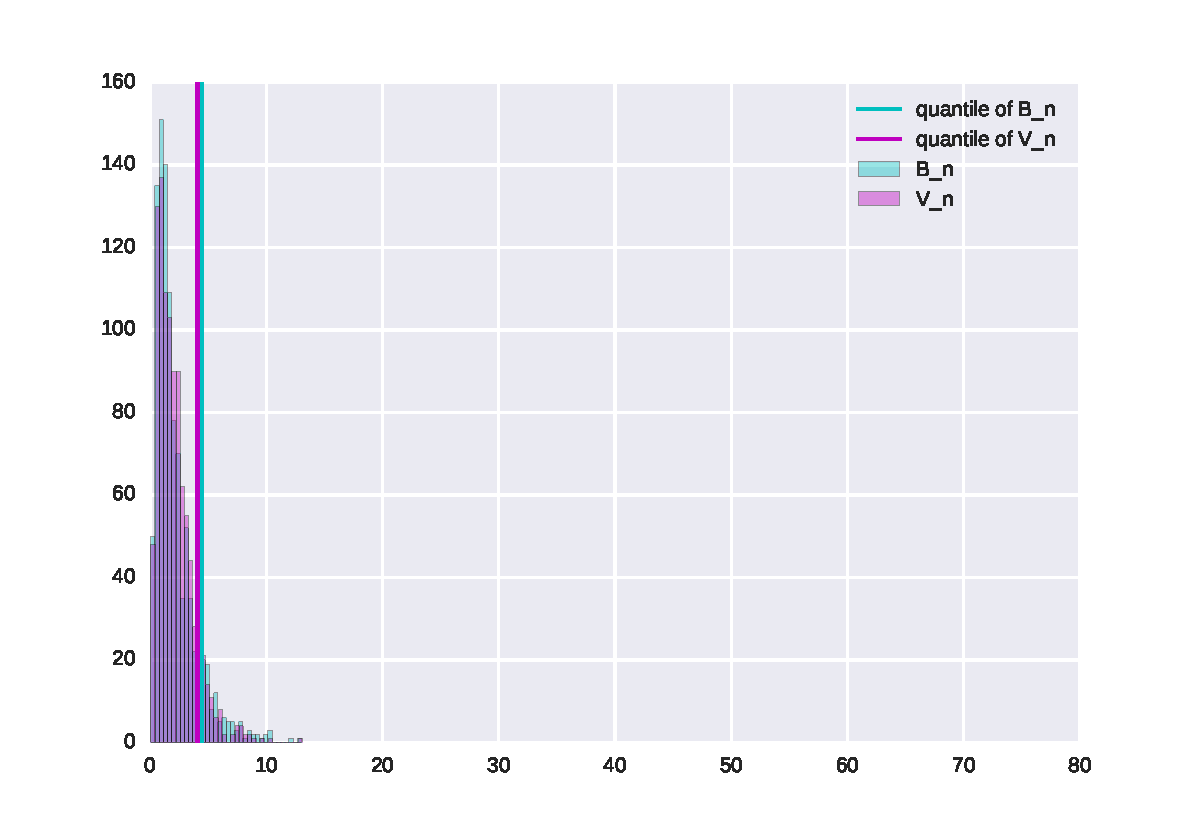
\includegraphics[width=0.3\textwidth]{./img/bootstrapWorks1.pdf}
 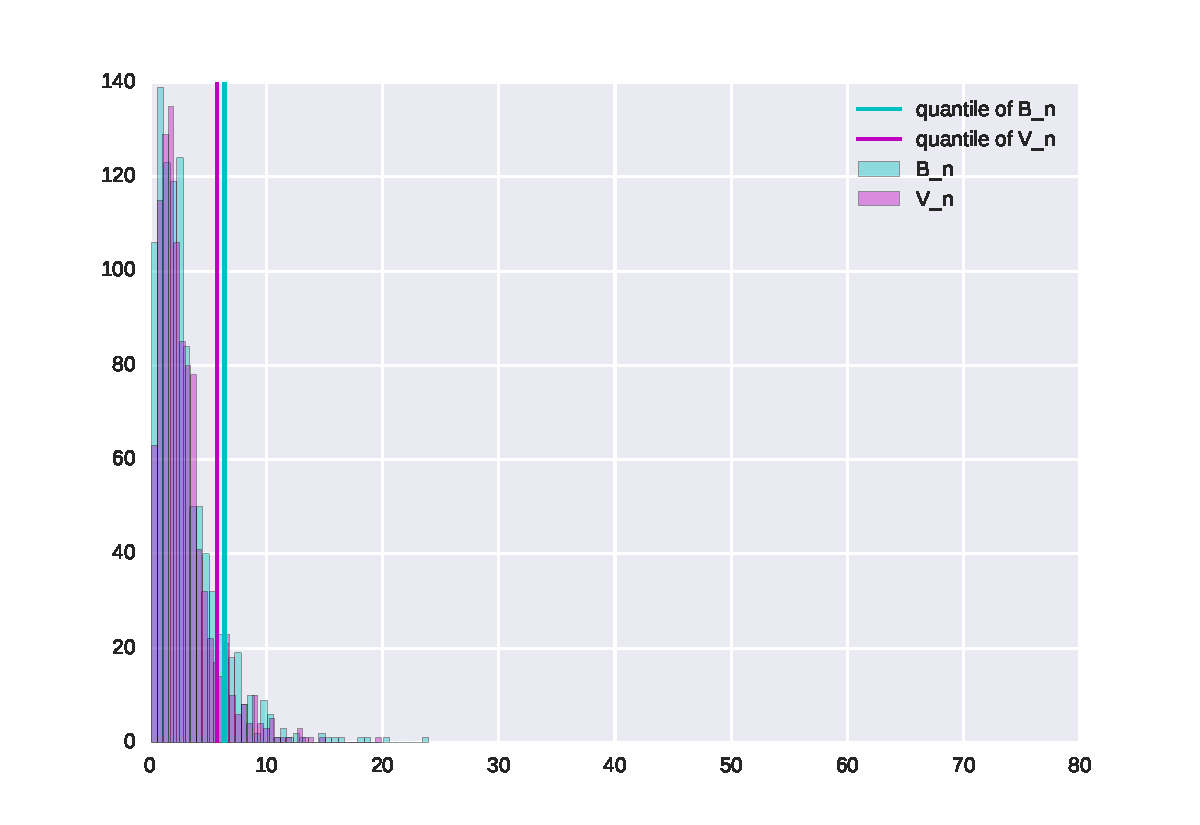
\includegraphics[width=0.3\textwidth]{./img/bootstrapWorks4.pdf}
 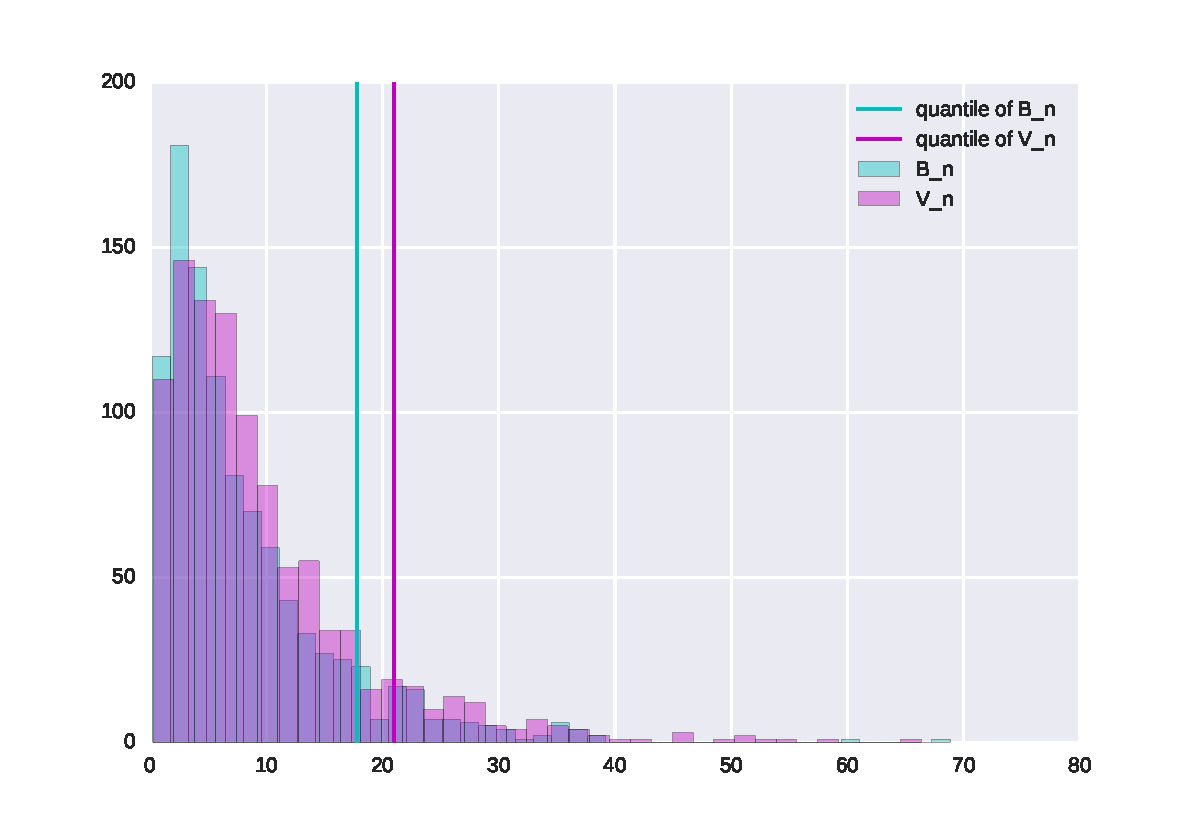
\includegraphics[width=0.3\textwidth]{./img/bootstrapWorks8.pdf}
\end{block}
\end{column}


% column 3
\hspace{-1.45cm}
\begin{column}{.32\linewidth}
\vspace{-0.75cm}
\begin{block}{Experiment: Student's T vs.\ Normal}
\begin{minipage}{.60\linewidth}
\begin{itemize}
\item TODO Describe
\end{itemize}
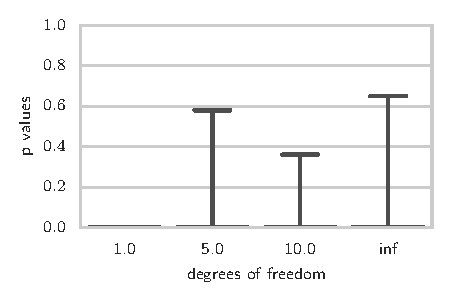
\includegraphics[width=.7\textwidth]{img/sgld_student_bad}
\end{minipage}
\begin{minipage}{.35\linewidth}
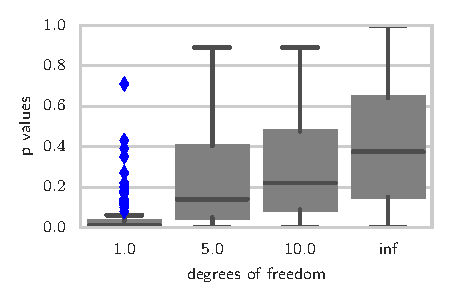
\includegraphics[width=1\textwidth]{img/sgld_student}\\
 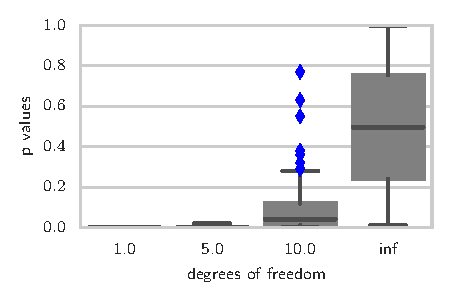
\includegraphics[width=1\textwidth]{img/sgld_student_opt} 
\end{minipage}
\end{block}
\vspace{-0.75cm}
\begin{block}{Experiment: Bias quantification in Approximate MCMC}
\begin{minipage}{.60\linewidth}
\begin{align*}
\theta_{1}\sim{\cal N}(0,10);\theta_{2}\sim{\cal N}(0,1)\\
X_{i}\sim\frac{1}{2}{\cal N}(\theta_{1},4)+\frac{1}{2}{\cal N}(\theta_{1}+\theta_{2},4) & .
\end{align*}
\begin{center}
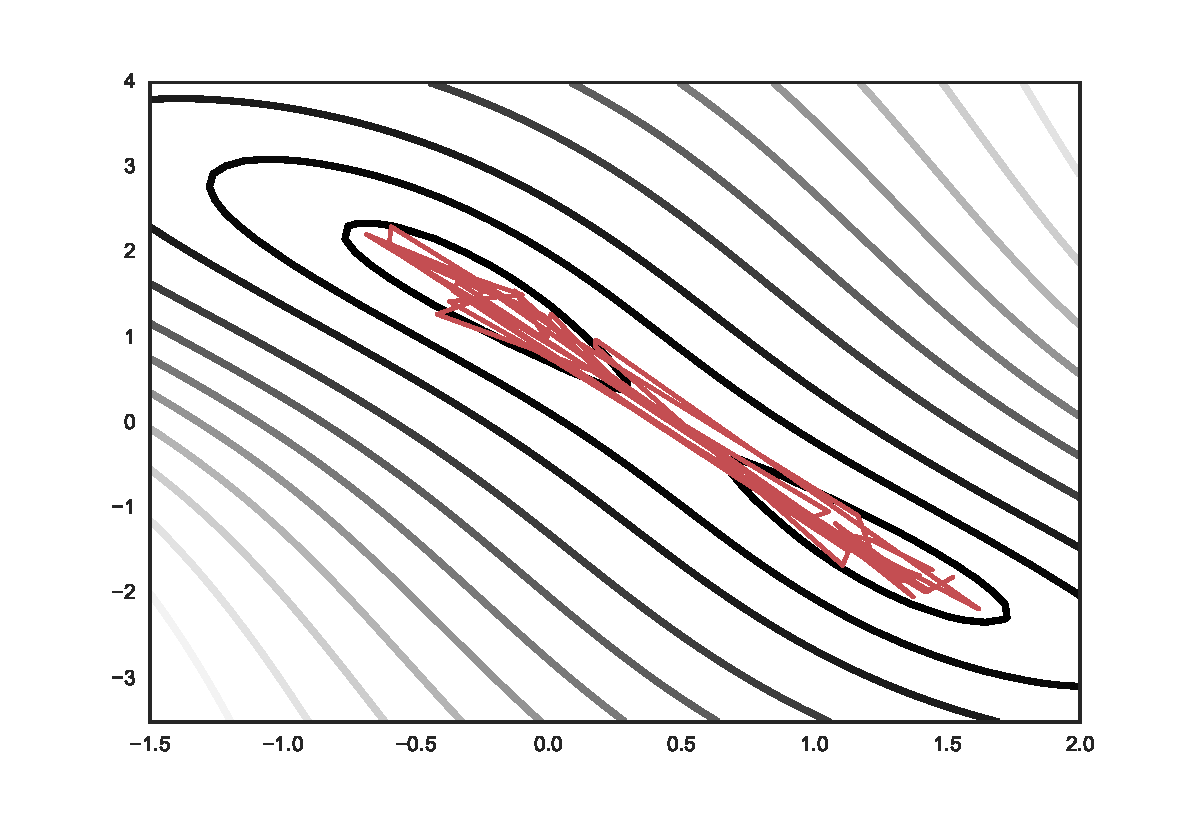
\includegraphics[width=0.5\textwidth]{img/sgld_trace_and_density.pdf}
\end{center}
\end{minipage}
\begin{minipage}{.35\linewidth}
           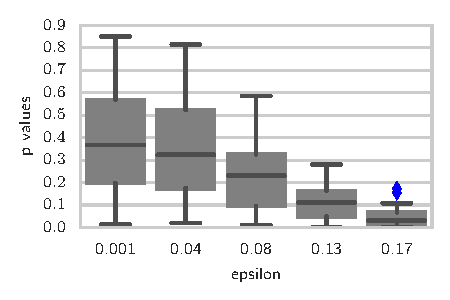
\includegraphics[width=.6\textwidth]{img/Heiko1}\\
            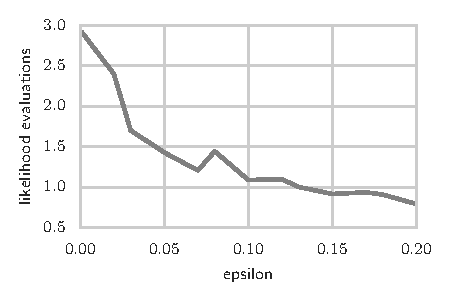
\includegraphics[width=.6\textwidth]{img/Heiko2}
\end{minipage}
\end{block}
\vspace{-0.75cm}
\begin{block}{Experiment: Statistical model criticism}
\begin{center}
\item We test the hypothesis that a Gaussian process generated {\color{red}training data} using for fitting -- without simulating from the generative model, but only using {\color{blue} test data}.
\end{center}
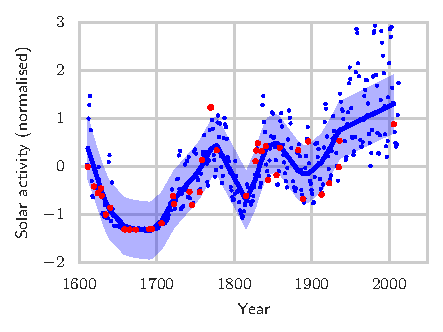
\includegraphics[width=0.48\textwidth]{img/gp_regression_data_fit.pdf} 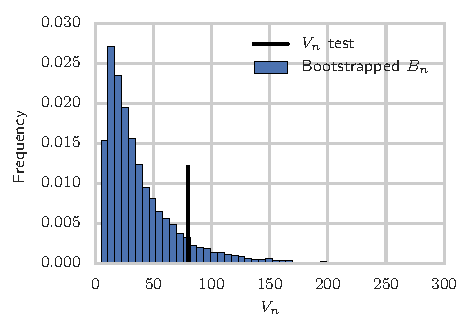
\includegraphics[width=0.48\textwidth]{img/gp_regression_bootstrap_hist} 
\begin{minipage}{.35\linewidth}

\end{minipage}
\end{block}
\vspace{-0.75cm}
\begin{block}{References}
\begin{minipage}{.9\linewidth}
{\footnotesize
\begin{multicols}{2}
\setbeamertemplate{bibliography item}[text] 
\bibliographystyle{plain} 
\scriptsize
\bibliography{../../biblio.bib} \ 
\end{multicols}
} 
\end{minipage}
\end{block}

\end{column}
\end{columns}

\end{frame}
\end{document}
